
Our contribution of the present work is to show that boosted regression tree models,
a powerful machine learning technique for function approximation, can meet the
requirements of this application.
We call this approach {\em predictive} auto-tuning to contrast it with the standard measurement-based approach which we will call {\em empirical} auto-tuning.
We show that the kernel from \citet{pinto+cox:2011gcg} can be modeled on a variety of hardware and get good performance compared to empirical auto-tuning.
%XXX: this has no flow

\iffalse
XXX: note that image processing libraries include convolutions (e.g. OpenCV ???
even for GPU!), but only don’t exploit the _bank_ dimension of the
_filterbank_ and thus can’t exploit parallel hardware as much.

XXX: in addition, when they are optimized, it’s often for pre-defined filters
(e.g. sobel?), and they are not suitable for encapsulation into libraries
usable by most real-world applications (bouuuuhhhh opencv !!!).
\fi

% %%%%%%%%%%%%%%%%%%%%%%%%%%%%%%%%%%%%%%%%%%%%%%%%%%%%%%%%%%%%%%%%%%%%%%%%%%%%%
\section{Discussion}

We're characterizing hardware by a 1-of-N feature vector, simply describing
which hardware is the current hardware.
To make better use of auto-tuning data from other platforms, it would be more
useful to have precise and descriptive features such as: what compute
capability is present, how many cores are active, what is the bandwidth
between the various kinds of memory, and how much of various kinds of memory
is present.  With these features a model-assisted auto-tuning approach
might be able to make very good guesses on hardware for which no auto-tuning
has ever been done.

In a complete implementation of Eq.~\ref{eq:z}, there would be parameters
related to the physical layout (e.g. strides) of $x$, $f$ and $z$ arrays in
addition to the mathematical parameters of heights and widths and so on,
so the total number of filterbank correlation computations that a user might
be able to demand is astronomical.
A typical coping mechanism would be to cast an arbitrary problem configuration into a more
standardized form, such as by copying inputs into aligned memory buffers with
appropriate padding, and then choosing an appropriate blocking strategy for
the computation. At that point, auto-tuning efforts can be focussed on the
kernel for each blocked strategy. However, on GPU hardware, the cost of
aligning the inputs can be relatively large.  In future work we hope to apply
our model-based technique to auto-tune in full problem configuration space, so
that we can optimize as much of the computation as possible within the
predictive auto-tuning framework (XXX name).

Platform Space: XXX

XXX: GCG chapter pg 13 notes that among the grid search, the best parameter
setting is different for the various platforms.

XXX: so far we only tried 3 cards... so we're using a 1-of-N feature.


%\renewcommand{\bibsection}{\section*{Bibliography}}
%\setlength{\bibsep}{5pt}



One might expect then, that it would be easy to implement a library providing
this operation -- this hypothetical library could have quite a simple interface
following the spirit of FFTW or a BLAS routine:
\begin{verbatim}
    gpu_fbcorr(
        img_shape, filters_shape,
        img, filters, output)
\end{verbatim}
However, as shown in \citet{pinto+cox:2011gcg} and numerous articles on
related stencil operations XXX, it is challenging to provide an implementation
or even an implementation strategy that provides satisfactory performance
across the range of inputs (shapes, physical layouts) that occur even in
typical usage.

Current state-of-the art is to do empirical auto-tuning.
XXX \vspace{12pt}

Increasingly, machine learning and statistical inference strategies are
finding application in compiler technology.
XXX \vspace{12pt}

machine learning

This paper shows that a kernel with several  boosted


There is a natural function from
problem space x implementation space x platform space to runtime:
how much wall time elapses on the given platform when solving the given
problem with the given implementation.

Auto-tuning is a family of empirical techniques for finding the implementation
that minimizes that runtime function, when the platform and the problem
configuration are given.

XXX: some math, or possibly a picture with the three boxes that was on Pinto's
whiteboard.

This paper is about different ways of doing the minimization.
For a particular problem (filterbank correlation) we
look at a parameterized kernel implementation (from \citet{pinto+cox:2011gcg})
and a few hardware platforms, and compare
random search, grid search, and a hill-climbing strategy with a good, but
generic, reference implementation.
Then we show that we can model the LSM function with a regression tree
well enough to usefully perform the argmin of Equation~\ref{eq:lsm_argmin}
on the model rather than the actual system. Whereas it may take several
minutes to perform a hill-climbing or grid search in the original system,
a hill-climbing search in the model requires a small fraction of a second.
Model-based autotuning makes it possible to simulate auto-tuning quickly and
accurately enough to be used within a single library call of the computational
routine.

Best arithmetic density

A bandwidth analysis that takes the blocking structure into account would
reveal that larger $H$ and $W$ require each block to read a larger input
region, and store it in a larger shared memory region, which reduces the
potential for high occupancy.

Filterbank correlation represents a difficult code-optimization problem
because of the number of interacting constraints: a large value of $P$ reduces
arithmetic density, but a small value of $P$ requires that each thread do more
work, and makes global memory access latency harder to hide. (XXX: is there a
better reason?)


The kernel used to perform
filterbank correlation was parametrized by 10 parameters, some of which
were binary and others of which were integer-valued. The full configuration
space included 12000 kernels.
XXX: how to make sense of these paramters without code listing?

XXX: What to all the parameters mean?
XXX: Point to github / GCG for full code listing.

XXX: how many configurations are in the configuration space

XXX: what was the reference kernel, and how was it chosen?

XXX: analysis of READ traffic, WRITE traffic, DATA re-use and CACHEing
strategies. FLOPS per write etc.

XXX: Why not use FFT: convolution in spectral domain?

XXXX: Talk about memory transfer requirements vs. speed vs. copy...

we believe that our approach is the most practial one to get high perf on
recent hardware, since there is no consensus on hw features (and it won't
change soon)

XXX: deliver significant performance increases at very low run-time cost (less
than a second if the input domain has not been seen before, zero if it
has, since it will hit the cache) compared with the reference
implementation

XXX always delivered good performance: optimality without loss of productivity?

XXX such machine learning derived model-based empirical auto-tuner hold great
promise for dev productivity, portability, performance on future multi-core hw
with different architectural features

XXX frameworks for predicting performance exist \cite{XXX}
% Hwu An Adaptive Performance Modeling Tool for GPU Architectures}
% but for non-GPU architectures

auto-tuning required hardward expertise *and* application-domain knowledge, we
want to remove these restrictions ultimately we want a ml-based approach to
code optimization that will where a set of generic but deep code
transformations, could be templated and injected in any domain-specific
library. this will reduce the need for specialized expertise across the range
of targetted computing systems.

\begin{figure}
\centering
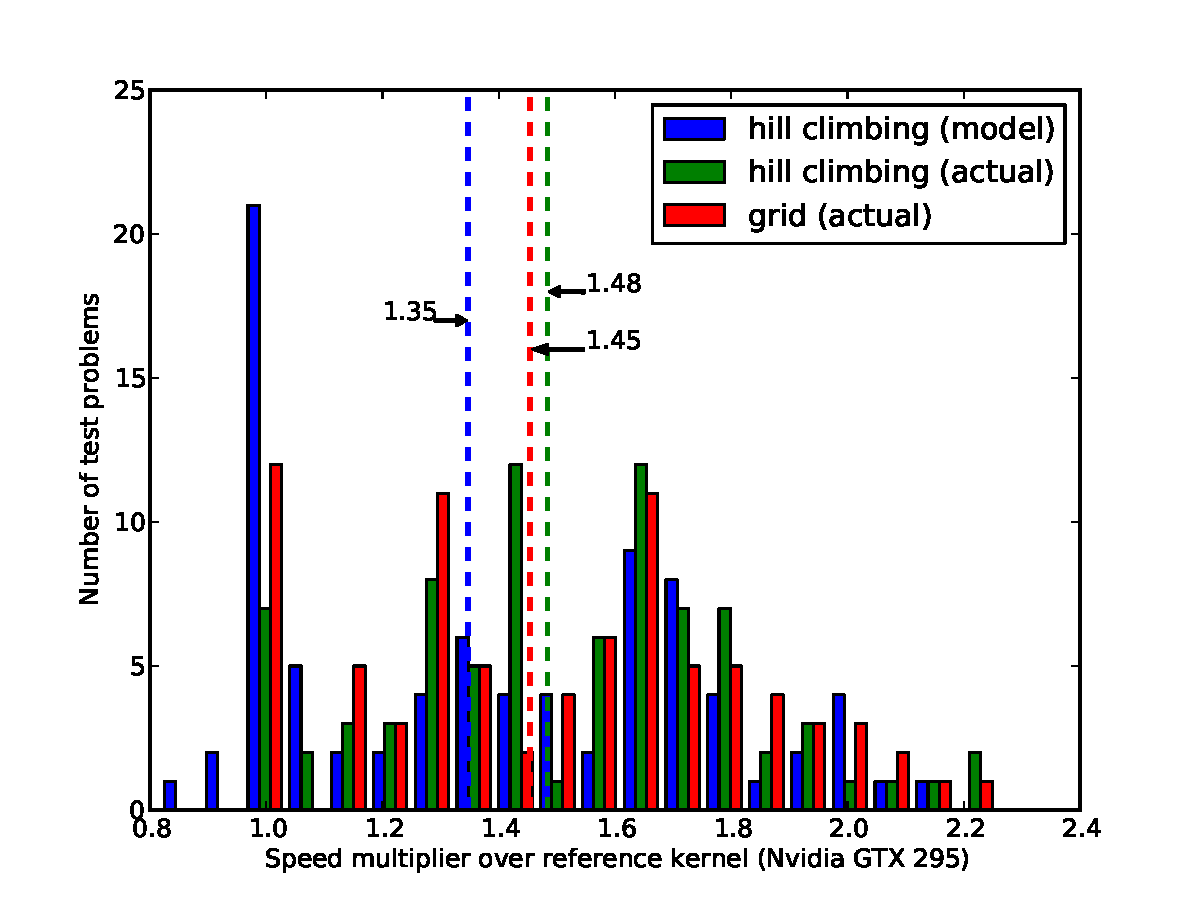
\includegraphics[scale=.42]{speedup_295.pdf}
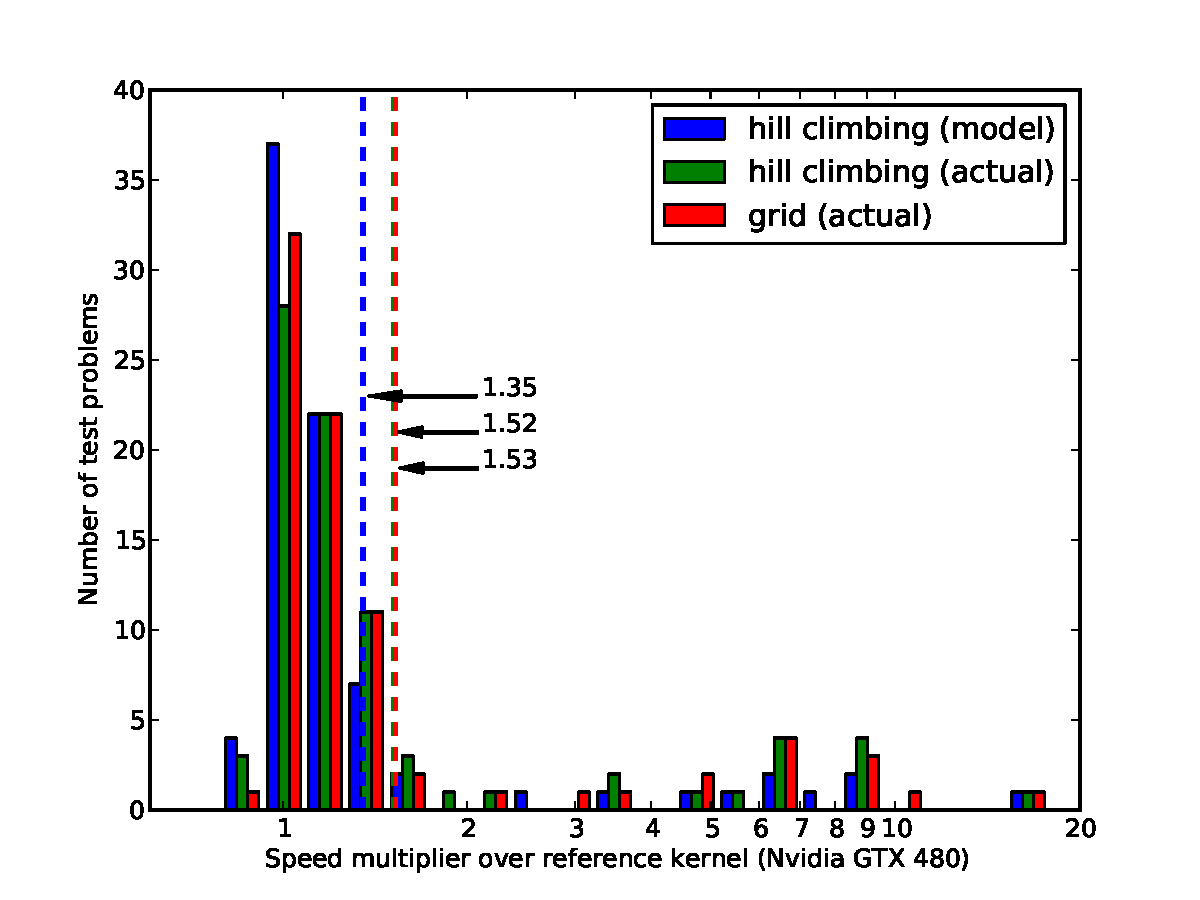
\includegraphics[scale=.42]{speedup_480.pdf}
\caption{
Speedup of various auto-tuning strategies over the reference
implementation.  Each strategy was evaluated the same set of 83 problem
configurations, which was disjoint from the problem configurations used
to build the model for model-based hill-climbing.  The vertical dashed
lines are positioned at the geometric mean speedup (XXX?) of each
strategy. The grid and hill-climbing approaches tested 73 and 75
configurations respectively, and took 45?? XXX seconds on average.
The model-based approach tested 0 configuration evaluations, and took 0.1
seconds on average, even with a naive Python implementation.
}
\label{fig:speedup}
\end{figure}

\begin{figure}
\centering
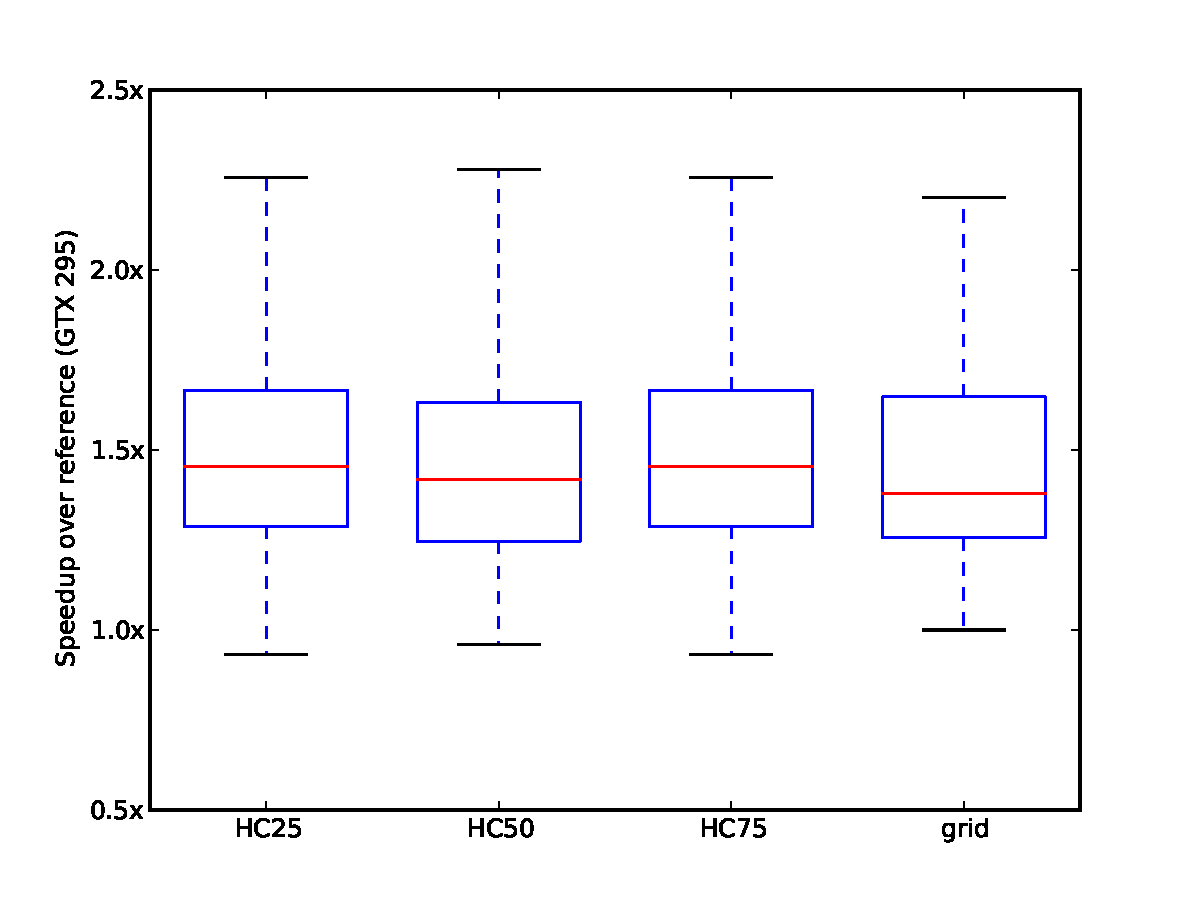
\includegraphics[scale=.42]{fig_genX_vader_295.pdf}
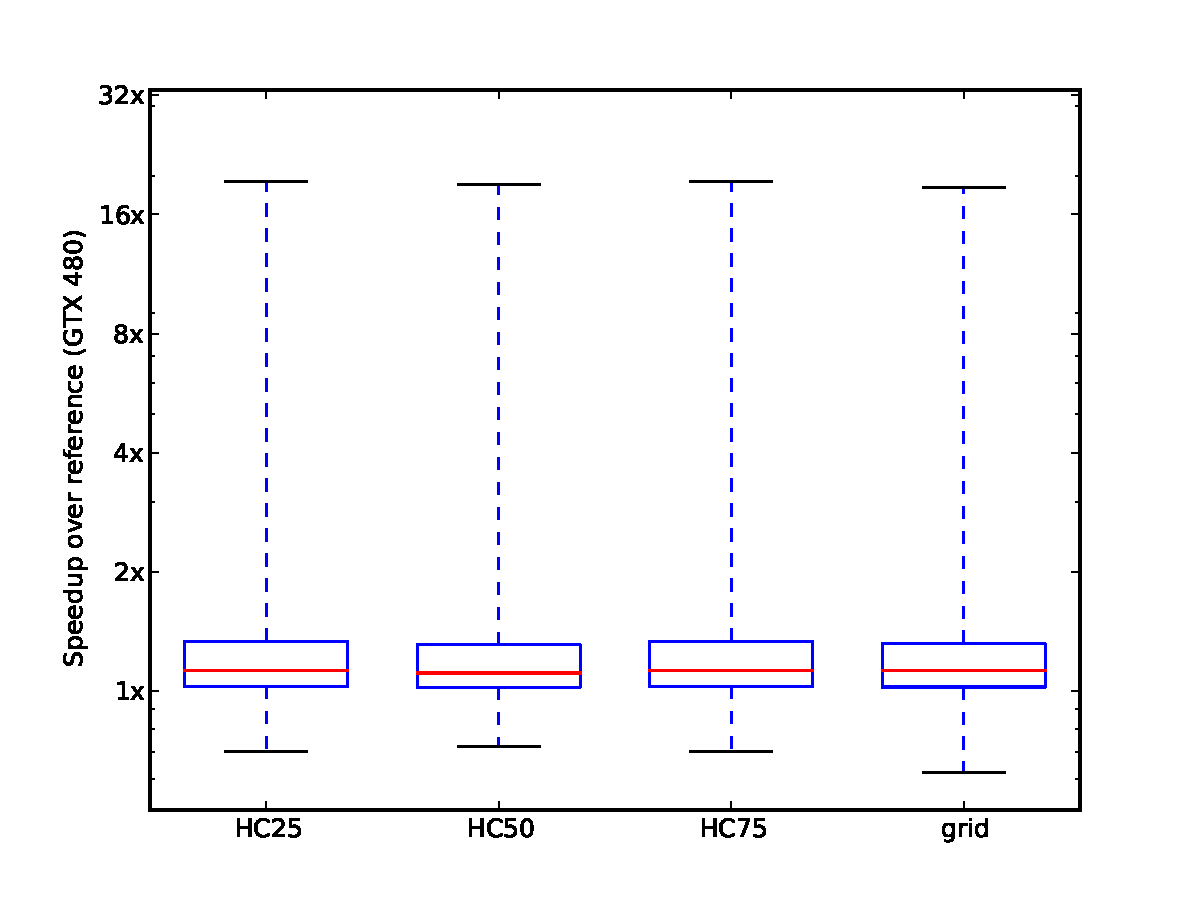
\includegraphics[scale=.42]{fig_genX_munctional0_480.pdf}
\caption{The speedup of hill-climbing (HC) and grid algorithms for empirical autotuning}
\label{fig:speedup}
\end{figure}

\begin{figure}
\centering
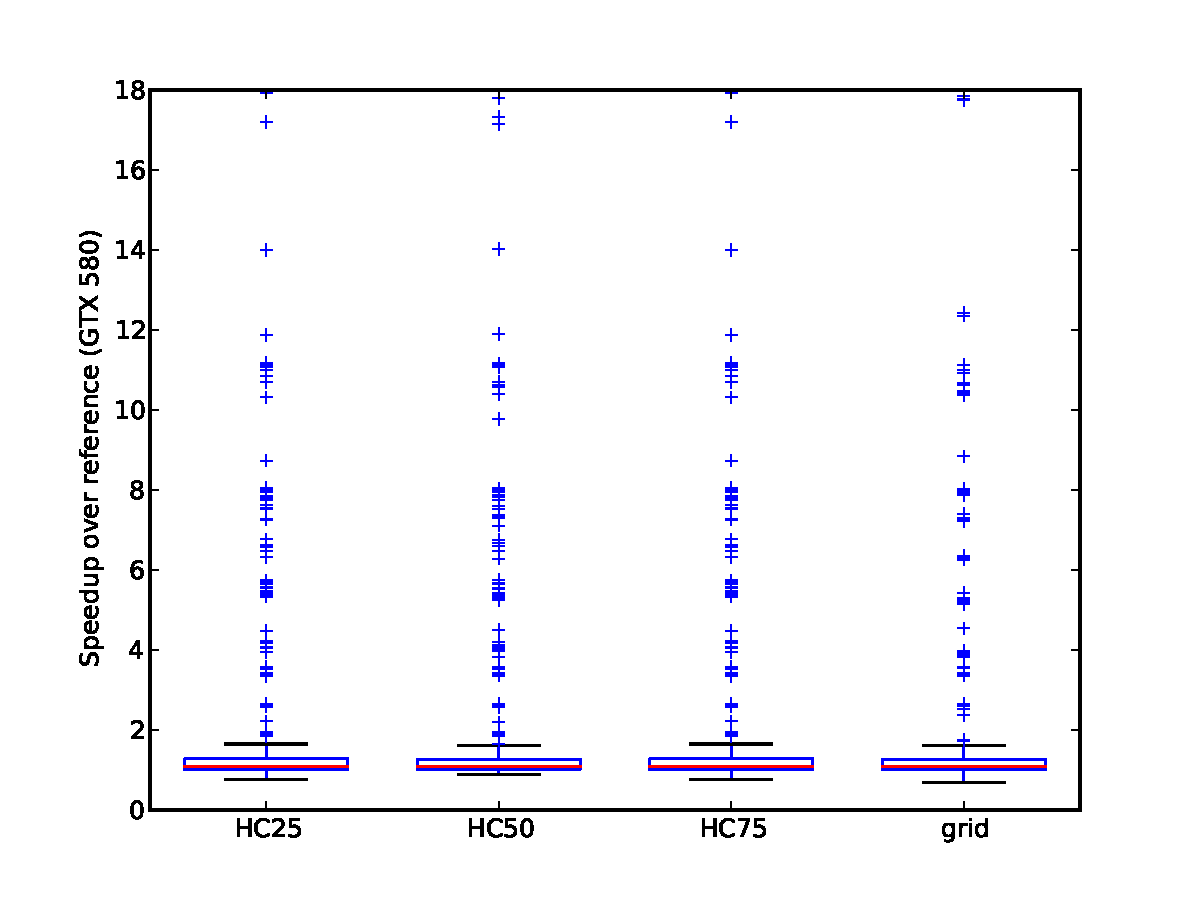
\includegraphics[scale=.42]{fig_genX_munctional0_580.pdf}
\caption{The speedup of hill-climbing (HC) and grid algorithms for empirical autotuning}
\label{fig:speedup}
\end{figure}

\begin{figure}
\centering
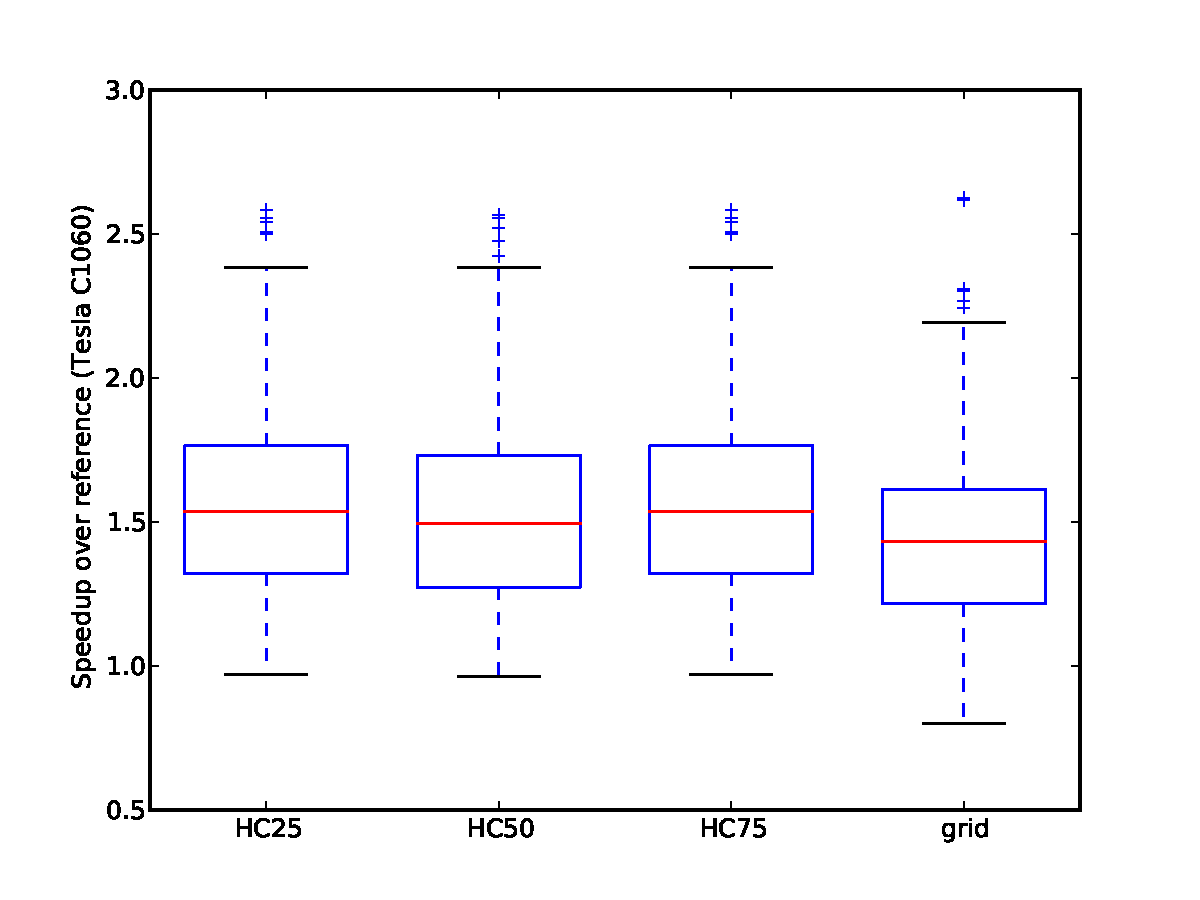
\includegraphics[scale=.42]{fig_genX_munctional0_1060.pdf}
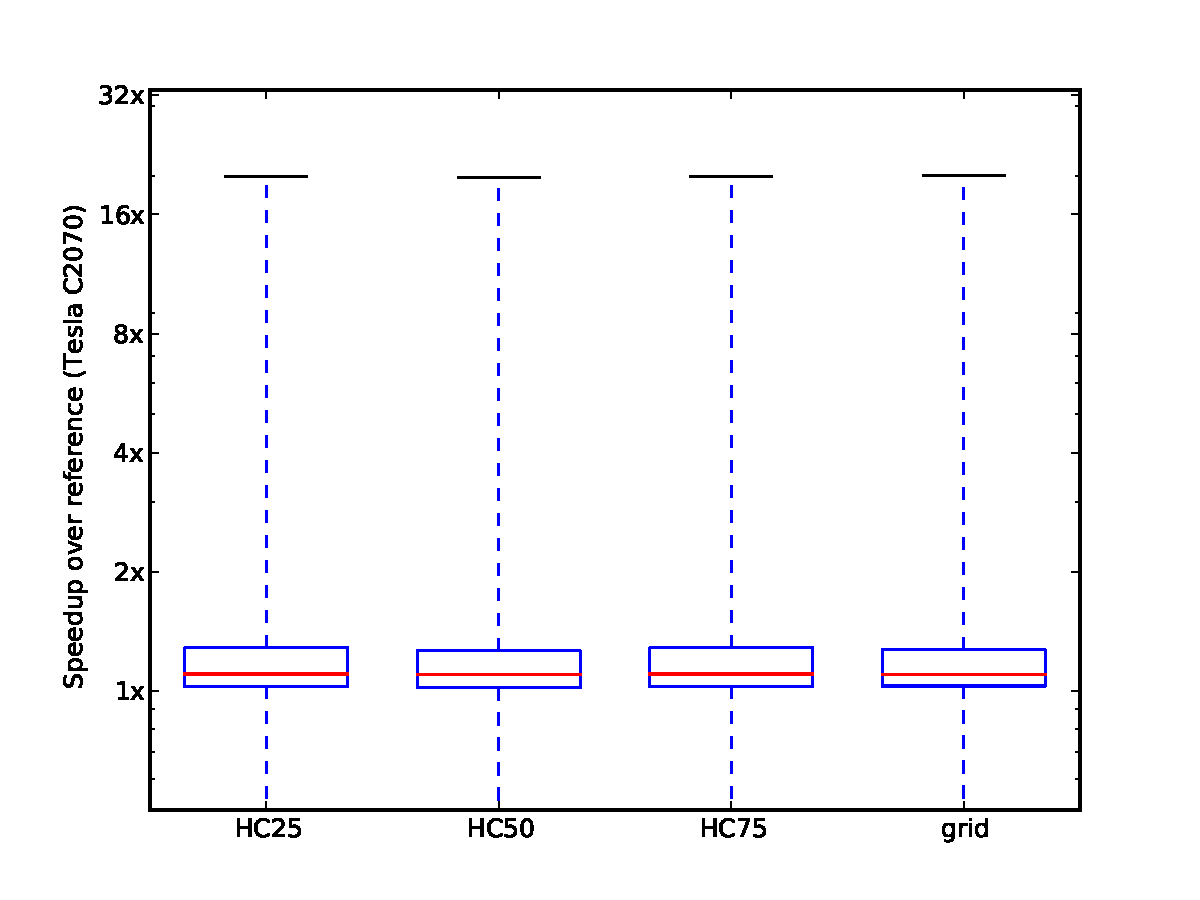
\includegraphics[scale=.42]{fig_genX_munctional0_2070.pdf}
\caption{The speedup of hill-climbing (HC) and grid algorithms for empirical autotuning}
\label{fig:speedup}
\end{figure}

